% Chapter 5
\chapter{Evaluation}\label{ch:eval}
\section{Experiments}
To select a benchmark cost a brute force search is performed on random generated test instances, evaluating a fixed number of trajectories. 
The time the algorithm needs to find this benchmark solution is used to compare their performance.

All algorithm are tested using different minimal, and maximal velocities to account for different acceleration limits. 

The weighting coefficients of the cost function are fixed to $\alpha=0.01$ and $\beta=1$. The local goal is also at a fixed location in the map. 
The step size of the collision test is fixed to 0.015 meter. 
Forward simulation time is fixed to one second. 

The following 60 test instances include different obstacle counts and random placement of quadratic obstacles:
\begin{itemize}
\item 15 instances with 1 obstacle and side length 1 meter.
\item 15 instances with 3 obstacles and side length 1 meter.
\item 15 instances with 5 obstacles and side length 0.5 meter.
\item 15 instances with 25 obstacles and side length 0.1 meter.
\end{itemize}

Figure~\ref{fig:fig_instances} illustrates three random instances. 
%\begin{figure}[thpb]
\begin{figure}[thpb]
     \footnotesize
      \centering
      \myfloatalign
      \setlength\fboxsep{0pt}
      \setlength\fboxrule{0.5pt}
       \subfloat[]
       {  
           \fbox{
\includegraphics[width=0.3\textwidth]{figures/01_1_b_nocost.png}}
       } 
       \subfloat[]
       {  
           \fbox{
\includegraphics[width=0.3\textwidth]{figures/03_5_m_nocost.png}}
       } 
       \subfloat[]
       {  
           \fbox{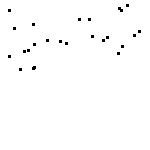
\includegraphics[width=0.3\textwidth]{figures/04_25_s_nocost.png}}
       }        
       \caption{Figures (a)-(c) show 3 out of 60 random instances for experiments. The instances differ in number and size of obstacles and are used for local costmap creation.}
      \label{fig:fig_instances}
   \end{figure}

The following list shows the tested algorithm:
\begin{itemize}
\item{\bf{Random Search with Tabu List:}} A repeated random guess of a velocity tuple $(v,w)$ (RST).
\item{\bf{Iterated Local Search:}} Performing Iterated Local Search with 4, 8 ,and 16 neighbors and Tabu List (ILS4, ILS8, ILS16).
\item{\bf{Variable Neighborhood Search:}} Variable Neighborhood search with Best-,and First-Improvement heuristic, and Tabu List (VNSB, VNSF).
\end{itemize}

\section{Test results}\label{sec:testresults}
\subsection{Overall Test}
In the first experiment the algorithms were applied to all 60 instances to evaluate a broad spectrum of possible environments. These tests were performed on a 2.4 GHz, Intel Core 2 Duo processor using 4 GB RAM.  
Figure~\ref{fig:fig_allworlds} illustrates the results using 240 trajectories, and using 2400 trajectory samples.
   \begin{figure}[thpb]
        \footnotesize
      \centering
      \def\svgwidth{\textwidth}
      \includesvg{figures/fig_allworlds}
      \caption{This figure shows the results of testing all 60 randomly generated instances. The top figure shows the run time performance for 240 trajectories, and the bottom figure for 2400 trajectories. Compared to brute force search, the Meta-Heuristic algorithms show a significant improvement. }
      \label{fig:fig_allworlds}
   \end{figure}

 
The results show that all algorithms, including RST, outperform the Brute Force generate-and-test method significantly. 
As expected increasing the number of trajectories greatly favors the Meta-Heuristic algorithms, since they benefit from larger search spaces. 
Notice that ILS and VNS algorithms differ apparently from the RST by exhibiting much smaller variance in their test results, indicating that randomization alone is not enough to achieve very good and stable performance.
Furthermore the VNS exhibit a more stable performance than the ILS methods. 
Comparing the ILS algorithms reveals the connection of the search space size to the size of the neighborhood. 
A small number of trajectories benefits smaller sized neighborhoods, whereas increasing the number of trajectories benefits larger neighborhoods. 

\subsection{Tests on specific instances}
The following tests only include the VNSF, VNSB and ILS4 algorithms. 
The algorithms are executed with specific world instances, and repeated 50 times. 
The results in Figure~\ref{fig:fig_special} show again that the VNS algorithms significantly outperform the Brute Force method. 

\begin{figure}[thb]
   \myfloatalign
   %\captionsetup[subfigure]{labelformat=empty} 
    \subfloat[]
    {  
       \def\svgwidth{\textwidth}
       \includesvg{figures/fig_6_40}
    }\\
    \subfloat[]
    {  
       \def\svgwidth{\textwidth}
       \includesvg{figures/fig_12_80}
    }
    \caption[Experiment: Trajectory size comparison]{The results of 50 consecutively executions with (a) 240 and (b) 960 trajectories, on particular instances which differ in number and size of obstacles. The blue line marks the run time for brute force search, which is used as a benchmark.}  
     \label{fig:fig_special}
\end{figure}
   
Analyzing the results of the ILS4 algorithms shows that a too small environment will quickly degrade to random search. 
Here the use of a neighborhood structure pays off and the VNS approaches perform evidently better than ILS. 
In addition, the results show that the algorithms perform good independent of number and size of obstacles.

\subsection{Tests comparing the influence of velocity bounds}

As for nearly all optimization problems, the No Free Lunch theorems \cite{wolpert1997no} apply to the local planning domain. 
Looking at all the results, there is no clear winner among the algorithms. 
Nevertheless using Variable Neighborhood search with Tabu List and Best Improvement heuristic seem to yields the best and most stable overall performance. 

In general the run time of the python implementation is not very efficient compared to tuned C++ implementations. 
Therefore the absolute numbers of the run time evaluations should be handled with care. 

\subsection{Tests on extending existing local planner}
